\section{Disc speeds}\label{sec:speed}

Over the course of its rotation, the wire will spend the vast majority of its time bathed in ambient air.  It will only be subjected to the intense heat of the oxyfuel flame for a brief interval.  This section is devoted to predicting how well such an arrangement will protect the wire from destruction due to melting.

A wire of diameter, $D_w$, length, $L$, with specific heat, $c$, and density, $\rho$, undergoing convection with a coefficient, $h$, will heat according to the equation
\begin{align}
\rho c \frac{L \pi D_w{^2}}{4} \dot{T} &= \pi D_w L h\left(T_{amb} - T\right).\nonumber
\end{align}
or simply
\begin{align}
\frac{\rho c D_w}{4 h} \dot{T} + T = T_{amb}.\label{eqn:Twire}
\end{align}
Nichrome steel enjoys a high mechanical strength, relatively high density (7,900 kg/m$^3$), relatively high specific heat (500J/kg-K) and favorable resistance to corrosion.  If the convective coefficient were aggressively approximated on the order of 1000W/m$^2$-K for a 0.25mm (0.01in) diameter wire, then the time constant, $\tau$, of Equation \ref{eqn:Twire} is about one quarter (0.25) seconds.

After sufficient time has passed that the wire has taken many journeys through the flame, its temperature prior to entering will converge to some constant, and the temperature response will converge to a piecewise solution.  If the wire is emersed in the flame for an interval, $t_f$, and requires $t_c$ seconds to rotate, then 
\begin{subequations}\label{eqn:T}
\begin{align}
\tau \dot{T} + T &= T_{flame} & 0 \le t < t_f\label{eqn:T:tf}\\
\tau \dot{T} + T &= T_{amb} & t_f \le t \le t_c\label{eqn:T:ta}
\end{align}
\end{subequations}
with the boundary condition that $T(0) = T(t_c)$.  It will become quite convenient to non-dimensionalize the temperatures by scaling
\begin{align}
k &= \frac{T - T_{amb}}{T_{flame} - T_{amb}}.
\end{align}
so equations \ref{eqn:T} become
\begin{subequations}
\begin{align}
\tau \dot{k} + k &= 1 & 0 \le t < t_f\label{eqn:k:tf}\\
\tau \dot{k} + k &= 0 & t_f \le t \le t_c\label{eqn:k:ta}
\end{align}
\end{subequations}

The solutions are
\begin{align}
k(t) = \left\{\begin{array}{lr}
(k_{min} - 1) \exp(-t/\tau) + 1 & \ 0 \le t < t_f\\
k_{max} \exp(-(t-t_f)/\tau) & \ t_f \le t \le t_c
\end{array}\right.
\end{align}
when $k_{min}$ and $k_{max}$ are the temperatures prior to and after the wire's passage through the flame respectively.  We solve for them by asserting that
\begin{align}
k_{max} &= (k_{min} - 1) \exp(-t_f/\tau) + 1\nonumber\\
k_{min} &= k_{max} \exp(-(t_c-t_f)/\tau)\nonumber
\end{align}
when $t_f$ is the time the wire dwells in the flame, $t_c$ is the period of rotation.  The time that the wire spends in the ambient, $t_a = t_c-t_f$, appears naturally.  Solving for $k_{min}$ and $k_{max}$, 
\begin{subequations}\label{eqn:k}
\begin{align}
k_{max} &= \frac{1-\exp(-t_f/\tau)}{1-\exp(-t_c/\tau)}\label{eqn:kmax}\\
k_{min} &= \frac{\exp(-t_a/\tau)-\exp(-t_c/\tau)}{1-\exp(-t_c/\tau)}\label{eqn:kmin}
\end{align}
\end{subequations}

The times, $t_c$, $t_a$, and $t_f$, are determined by the rotation frequency, $f$ and the fraction, $\chi = t_f / t_c$, of the disc's motion that places the wire in the flame.
\begin{align}
t_c = \frac{1}{f} & & t_f = \frac{\chi}{f} & & t_a = \frac{1-\chi}{f}\nonumber
\end{align}
We may expand the exponentials of equation \ref{eqn:kmax} to obtain a simpler estimate for the maximum temperature,
\begin{align}
k_{max} \approx \chi \frac{2f\tau - \chi}{2f\tau - 1}\label{eqn:kmax:lim}.
\end{align}
Clearly, in the limit where $f\tau \gg 1$, $k_{max} \rightarrow \chi$.

Figure \ref{fig:convection} shows the dimensionless temperatures $k_{max}$ and $k_{min}$ versus disc speed, and the approximate $k_{max}$ is plotted with a dashed line.  The choice of $\chi=0.2$ is consistent with a flame approximately 12mm (0.5in) across with a wire radius of 100mm (4in).

\begin{figure}
\begin{center}
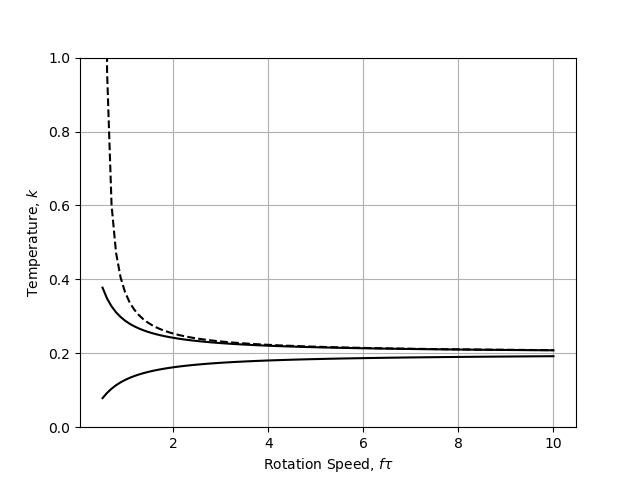
\includegraphics[width=0.9\linewidth]{convection.png}
\caption{Maximum and minimum d-less temperatures versus d-less disc speed for $\chi=0.2$.  The dashed line is the approximate $k_{max}$ from Equation \ref{eqn:kmax:lim}}\label{fig:convection}
\end{center}
\end{figure}

Since $\chi$ will be constant for a given flame and disc geometry, and $k_{max}$ is a constraint based on the melting temperature of the wire, we may calculate a minimum safe disc speed.  When we use the expansion in Equation \ref{eqn:kmax:lim}, we will produce a conservative calculation for $f$ that cannot be less than $1/2\tau$ due to the singularity in the expansion.
\begin{align}
f > \left(\frac{1}{2\tau}\right)\left(\frac{k_{max}-\chi^2}{k_{max}-\chi}\right)
\end{align}

If the flame temperature were about 3000K, the wire melting temperature were about 1700K, and the ambient were about 300K, then $k_{max} = 0.52$, and the minimum disc speed is $f > 0.75 / \tau$.  If $\tau$ is 0.25s, then the disc should spin at least three rotations per second (180rpm).

While this is a modest speed for a spinning disc, it should be emphasized that the estimates for the peak wire temperature may be regarded as quite aggressive.  Firstly, all additional cooling due to radiation or conduction along the wire length have been neglected.  Moreover, the expansion used in forming Equation \ref{eqn:kmax:lim} is inherently pessimistic as shown in Figure \ref{fig:convection}.  The only cause for concern that higher wire temperatures may be possible seems to be that the convection in the flame could be more severe than the convection in the ambient.

Regardless, a 200mm (8in) diameter disc spinning at about 70 revolutions per second (about 400rpm) should be far in excess of what is required to protect a 0.25mm (.01in) diameter wire.  Such a system would propel the wire at roughly 4.3m/s (170in/s), which is safely less than the velocities that are likely in the flame.  

The current signal that should be generated by such an experiment should form a pedestal with a width determined by the wire's duration in the flame, and with internal features determined by the length scale of the flame's micro-structures.  If the wire processes with a speed of 4.3m/s (170in/s) through a 12mm (0.5in) flame, then the pedestal is approximately 2.8ms wide.  The micro-structures that need to be resolved are probably determined by the number of individual flamelets formed at the tip's preheat openings.  If we were to assume that these were so tightly spaced as 1mm, then the pedestal will contain features as fast as 0.2ms.

Time scales between 2.8ms and 0.2ms correspond to frequency content from 300Hz to 5kHz.  Of course, these frequencies will scale with the disc speed.  If these settings are respected, digital sampling must be \emph{at least} 10kHz, and filtration below 5kHz must be avoided.

Were the diameter of the wire halved, so would the wire's thermal time constant, and the minimum disc speed would double.  Because 400rpm was already an aggressive choice for a 0.25mm (.01in) wire, it should still be acceptable for a 0.12mm (.005in) diameter wire.

